\documentclass[handout]{beamer}

\usepackage[english]{babel}
\usepackage[latin1]{inputenc}
\usepackage[T1]{fontenc}
\usepackage{graphicx}
\usepackage{geometry}
\usepackage{amsmath,amssymb}
\usepackage{epstopdf}
\usepackage{url}



%\usetheme{Marburg}
%\usetheme{Berkeley}
\usetheme{PaloAlto}
%\usetheme{Warsaw}


\AtBeginSection[]
{
  \begin{frame}
  \frametitle{Sommaire}
  \tableofcontents[currentsection, hideothersubsections, pausesubsections]
  \end{frame} 
}



\title{\textbf{Top-Down and Bottom-up Cues for Scene Text Recognition}}
\author{Vincent BODIN \& Thomas MOREAU}




\begin{document}

\renewcommand{\contentsname}{Sommaire}


\begin{frame}[allowframebreaks]
\titlepage
\end{frame}


\section*{Introduction}


\begin{frame}{Introduction}
\begin{itemize}
	\item Robust methods have allowed recognizing letters efficiently recently (OCR).
	\item Scene text recognition has been a center of interest in computer vision for those few last years. 
	\item We decided to implement a paper by A. Mishra, K. Alahari, C. V. Jawahar, \emph{Top-down and Bottom-up Cues for Scene Text Recognition} \cite{Mis}
\end{itemize}
\end{frame}




\section{Learning preliminaries}

\subsection{Learning characters}

\begin{frame}{Learning characters}
We need to build classifiers to recognize characters in a natural picture:
\begin{enumerate}
	\item Use a database to identify characters: ICDAR 2003 \cite{ICDARchar}, Chars74K \cite{Char74K};
	
	\item extract features: Histogram Of Gradient (HOG) \cite{Dal2005}\footnote{N. Dalal, B. Triggs, Histogram of oriented gradients for human detectection};
	
	\item build $K$ SVMs ($K$ is the number of classes, 62) with RBF Kernel, Fig.(\ref{RBFKernel}):
	\begin{equation}
	\exp(-\gamma |x-x'|^2), \gamma > 0
	\label{eq:}
	\end{equation}
	method one-versus-all, we used a Python librairy scikit-learn \cite{scikit}: two parameters $\gamma$ and regularization $C$ optimized by cross-validation -> test error without optimization $25\%$, with optimization $16\%$.
\end{enumerate}
\end{frame}


\begin{frame}
\begin{figure}%
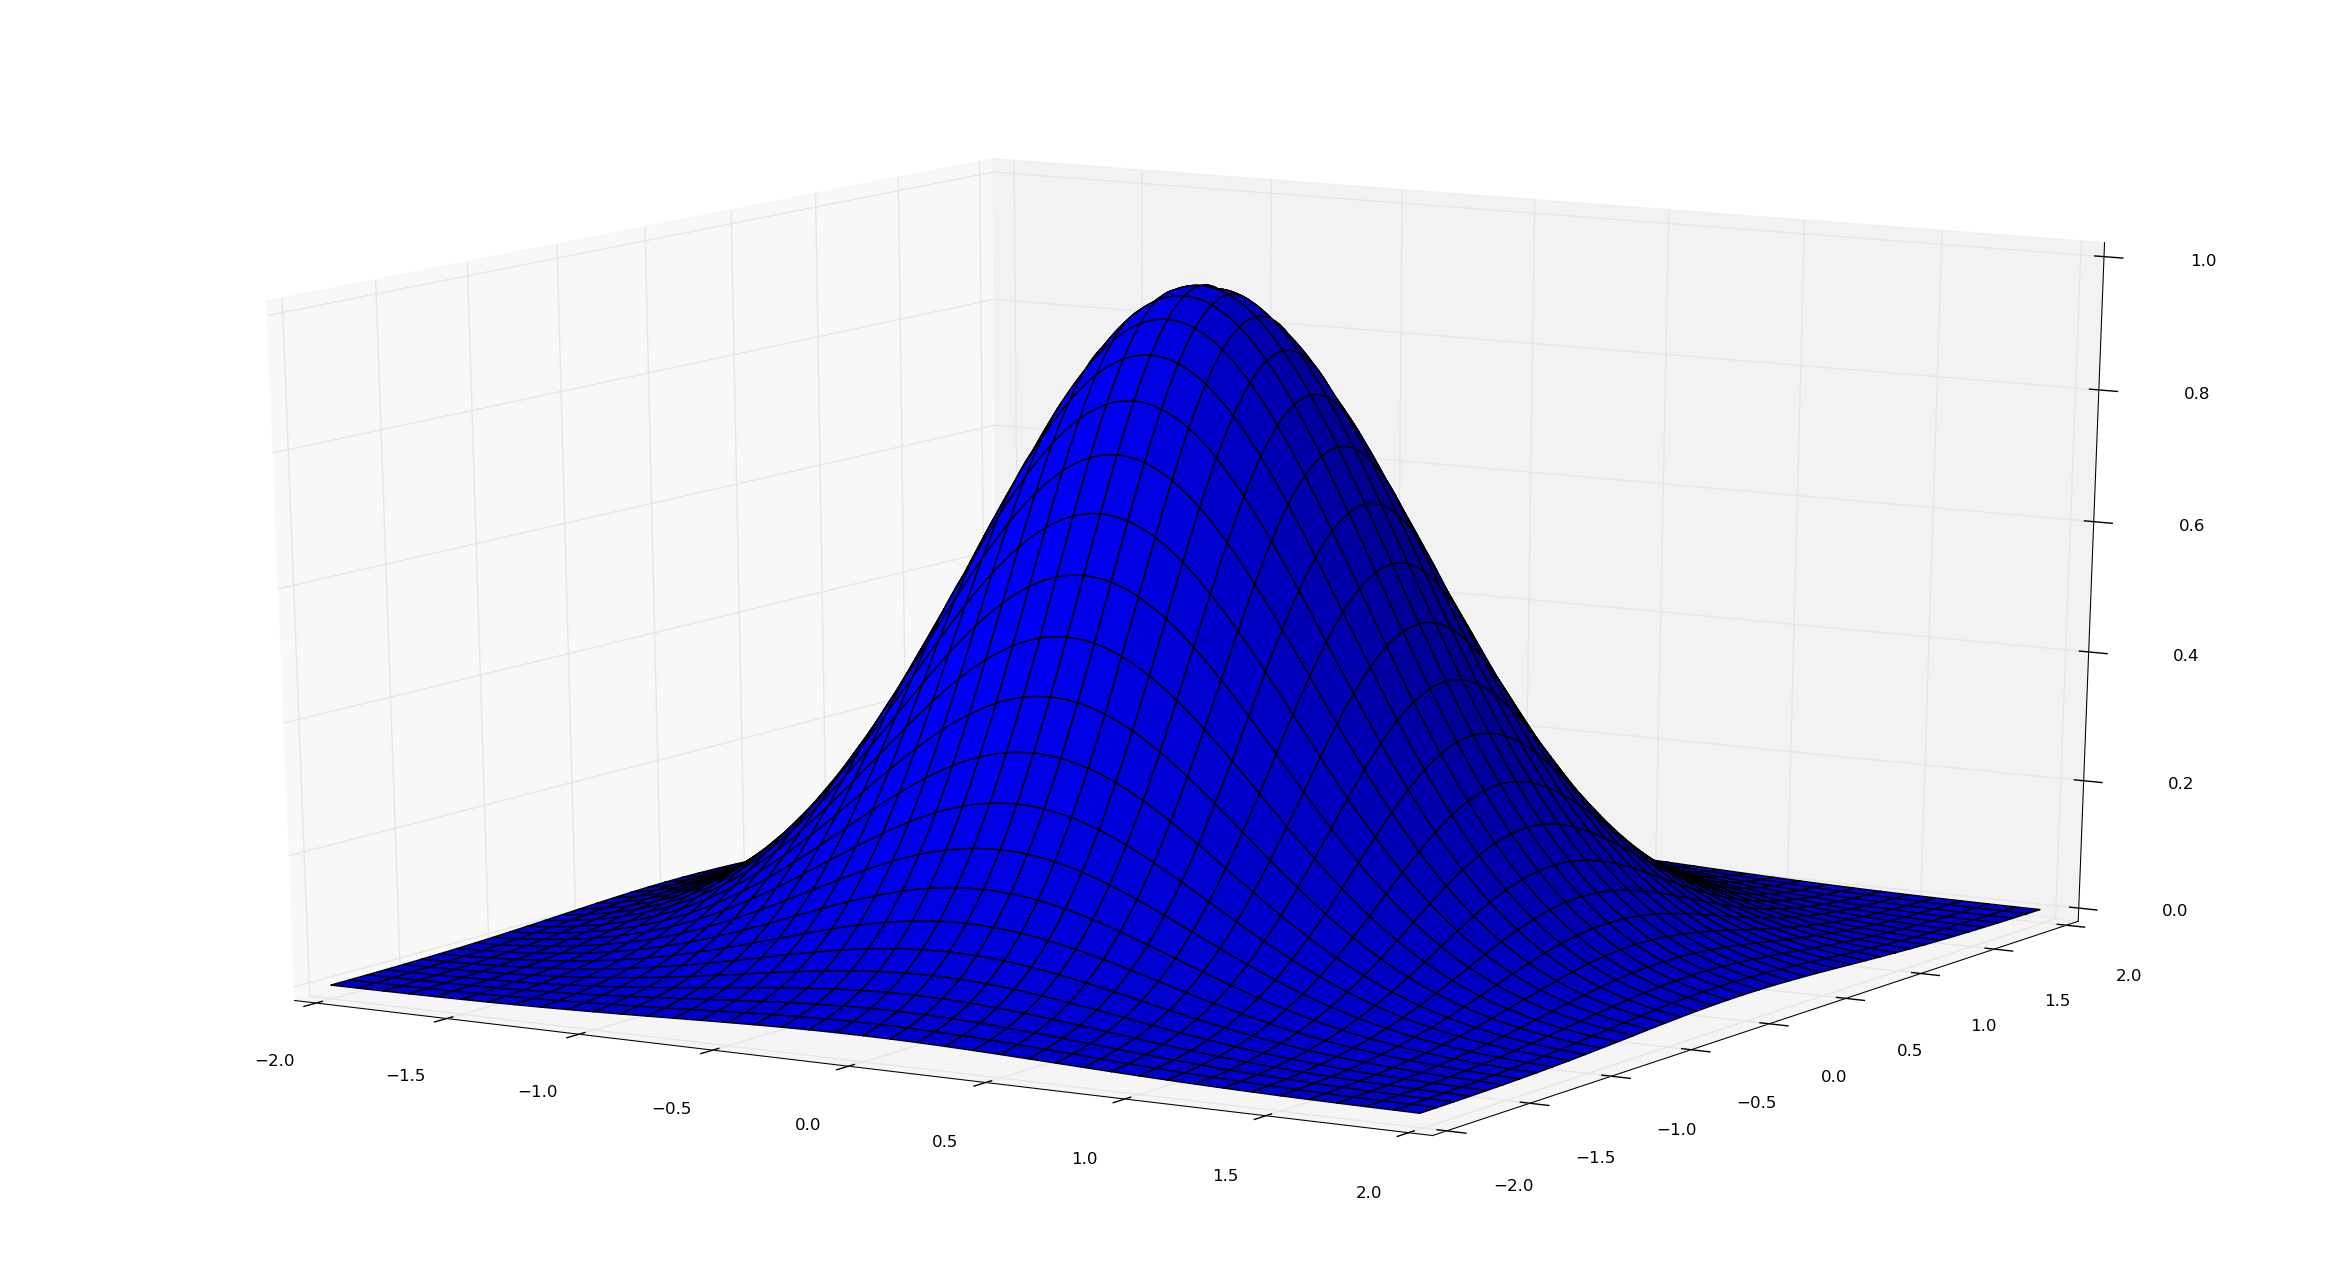
\includegraphics[width=\columnwidth]{figures/blob.png}%
\caption{RBF Kernel}%
\label{RBFKernel}%
\end{figure}
\end{frame}



\subsection{Learning words}

\begin{frame}{Learning words}
We have to build a prior lexicon that contains how characters interact to create words.
\begin{enumerate}
	\item Load a database of words \cite{ICDARword}\footnote{\url{http://algoval.essex.ac.uk/icdar/Datasets.html}};
	\item count for each pair of characters $(c_i,c_j)$ their frequency of occurrence $p(c_i,c_j)$ in the database (bi-gram model);
	\item will be used as an energy term to be minimized afterwards.
\end{enumerate}
\end{frame}





\section{Character detection}

%\subsection{Sliding window and pruning}

\begin{frame}{Sliding window and pruning}
\begin{itemize}
	\item Characters retrieved by sliding windows of different scales scanning the image;
	\item for each window $l_i$, compute the features $\phi_i$ of HOG with 12 orientations;
	\item run the 62 SVMs on $\phi_i$ and compute the goodness score:
	\begin{equation}
	GS(l_i) = \max_c p(c|\phi_i) \exp\left( - \frac{(a_i - \mu_{a_j})^2}{2\sigma_{a_j}^2} \right)
	\label{eq:}
	\end{equation}
	where $a$ is the aspect ratio and $j$ is the class that reaches the maximum \emph{i.e.} the index of the character that has the highest probability of being in this window.
\end{itemize}
\end{frame}

\begin{frame}{Sliding window and pruning}
\begin{itemize}
	\item if $GS(l_i) > 0.1$ then we keep the window \emph{and} all the probabilities of each character.
	\item apply Non-Maximum Suppression algorithm (NMS) to merge windows that overlap:
	\begin{enumerate}
		\item find the window with maximum confidence, say $l_i$.
		\item for all others $l_j$ compute:
		\begin{equation}
		\text{criterion} = \frac{l_i \cap l_j}{l_i \cup l_j}
		\label{eq:}
		\end{equation}
		\item if criterion > \texttt{threshold} then merge the windows.
		\item the ending merged window has the highest confidence and is located at the barycenter of all the windows merged.
	\end{enumerate}
\end{itemize}
\end{frame}


\section{Recognizing words}


\begin{frame}{Graph construction}
\begin{alertblock}{}
This part of the paper is implemented for the course of PGM, we will be brief!
\end{alertblock}
Suppose we are given a set of $n$ windows with possible characters inside.
\begin{enumerate}
	\item for each sliding window assign a node that takes values in $\mathcal{K}_{\epsilon}^n$ (add $\epsilon$ void label);
	\item build edges if the windows are 'close enough';
	\item assign unary energy to each node, and pairwise energy for edges composed of a term of overlapping and lexicon prior;
	\item minimize the discrete energy on the graph (NP-hard) with TRW-S algorithm \cite{Kol}.
\end{enumerate}

\end{frame}




\section{Implementation and first results}

\begin{frame}{Implementation and first results}
\begin{figure}%

\includegraphics[width=\columnwidth]{figures/puffTest.png}%
\caption{Image for testing the algorithm}%
\label{}%
\end{figure}
\end{frame}

\begin{frame}{Implementation and first results}
\begin{figure}%

\includegraphics[width=\columnwidth]{figures/puff.png}%
\caption{Word retrieved: 'PE'}%
\label{}%
\end{figure}
\end{frame}







\begin{frame}{References}
\tiny
\bibliographystyle{unsrt}
\bibliography{biblio}
\end{frame}






\end{document}